\documentclass[12pt]{article}
\usepackage{color}
\usepackage{graphicx}
\usepackage{booktabs}
\usepackage{amsmath}
\usepackage[utf8]{inputenc}
%\usepackage[german]{babel}
\usepackage{multirow}
\usepackage{siunitx}
\usepackage{pbox}
%\usepackage{tabularx}
\usepackage{multirow}
\usepackage{float}
%% ermöglicht Unter-Bilder in einer figure-Umgebung
\usepackage{subcaption}
\usepackage{amssymb,amsmath}
\graphicspath{{figures/}}
\makeatletter
\def\maketag@@@#1{\hbox{\m@th\normalfont\normalsize#1}}
\makeatother
\setlength{\parindent}{0pt}

%\addtolength{\textwidth}{1in}
%\addtolength{\textheight}{1in}
%\addtolength{\evensidemargin}{0.5in}
%\addtolength{\oddsidemargin}{-0.5in}
%\addtolength{\topmargin}{-0.6in}
%\addtolength{\bottommargin}{0.4in}


\usepackage[top = 2.50cm, bottom = 2.50cm, left = 2.75cm, right = 2.50cm]{geometry}

\usepackage[
 pdftex,                        % wir verwenden pdftex/pdflatex
 bookmarks=true,                % wir wollen auch im PDF-Reader ein Inhaltsverzeichnis
 bookmarksdepth=3,              % das Inhaltsverzeichnis soll 3 Tiefen enthalten
 colorlinks=true,               % Linktexte sollen Farbig sein
 linkcolor=black,               % Links innerhalb des Dokuments bleiben schwarz
 citecolor=black,               % Links zu Quellenangaben bleiben ebenfalls schwarz
 urlcolor=blue,                 % URL-Linktexte sollen blau dargestellt werden
%  pdfborder={0 0 0}              % Links im PDF erhalten keinen Rahmen, nur nötig wenn colorlinks=false
]{hyperref}

\usepackage[english, capitalise]{cleveref} %% definiert \cref: Referenzen mit korrekter Bezeichnung (z.B. "Abbildung 1") | die Nummer alleine ist weiter mittels \ref verfügbar | muss NACH 'hyperref' geladen werden

\renewcommand{\floatpagefraction}{1.0}


\begin{document}
\title{PHY118/119 \\ {\bf Newton'sche Mechanik}}
\author{Autor: Simon Flury \\ Co-Autoren: Nik Dennler, Johannes Lade \\ E-mail: simon.flury@uzh.ch \\\\ }
\maketitle

\section{Achtung!}
Dieses Dokument ist kein offizielles Vorlesungsmaterial. Es wurde weder von Prof. Kilminster noch vom Hauptassistenten abgesegnet, somit kann sich nicht darauf bezogen werden und es wird auch keine Haftung für Fehler übernommen. Es soll einzig und allein der Lernunterstützung dienen und bezieht sich ausschliesslich auf unsere Übungsstunden.

\section{Starre Körper}
Ein starrer Körper im Sinne der klassischen Mechanik beschreibt ein Modell eines nicht verformbaren Körpers. In der Realität verformt sich jedes Objekt ein wenig, jedoch meist nur soviel, dass wir die Verformung vernachlässigen können und die Behandlung als idealisierten starren Körper gute Näherungen liefert. Der Körper an sich muss nicht zwingend eine kontinuierliche Massenverteilung aufweisen, sondern kann auch ein System von einzelnen Massenpunkten sein.\\
\\
\subsection{Definition}
Bei einem starren Körper bleiben die Abstände zwischen den einzelnen Molekülen konstant:
\begin{equation}
d = |\vec{r_i} - \vec{r_j}| = \mathrm{const}
\end{equation}

\newpage
\subsection{Aufteilung der Bewegung in Translation und Rotation}


\paragraph{Translation:}
Bei der reinen Translation gibt eine beliebige Geschwindigkeit in einem Punkt des Körpers die Translationsgeschwindigkeit des ganzen Körpers an, da sie (wieder aufgrund der Invarianz der Abstände) als Schwerpunktsgeschwindigkeit aufgefasst werden kann: 
\begin{equation}
\vec{v_i} = \vec{v_s} \qquad \forall i \in \mathbb{N}
\end{equation}

\begin{figure}[H]
  \centering{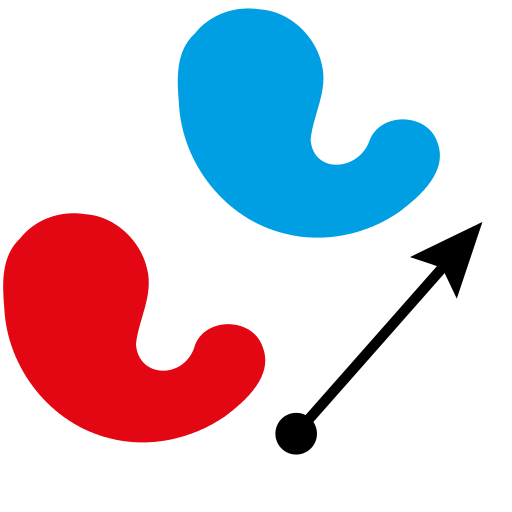
\includegraphics[width=0.15\textwidth]{Grafik2_2.png}}
  \label{fig:1teil}
\end{figure} 


\paragraph{Rotation:}
Wir betrachten eine reine Rotationsbewegung um eine feste Rotationsachse. Betrachte den zeitabhängigen Winkel $\varphi (t)$. Der Betrag der Winkelgeschwindigkeit (bzw. die Kreisfrequenz) ist gegeben durch 

\begin{equation}
 \omega = \dfrac{d \varphi}{dt} = \dfrac{2\pi}{T}.
\end{equation}

Da wir im Modell des starren Körpers die Abstände als fix betrachten, gilt: \\
\underline{Die Winkelgeschwindigkeit ist überall gleich.} \\\\
Vektoriell betrachtet ist die Winkelgeschwindigkeit gegeben durch 
\begin{equation}
 \vec{\omega} = \dfrac{d \varphi}{dt} \ \vec{u},
\end{equation}
wobei $\vec{u}$ ein Einheitsvektor (Vektor mit Länge 1) ist, der in die gleiche Richtung zeigt wie die Rotationsachse.
Es folgt für die Geschwindigkeit:
\begin{equation}
\vec{v} = \vec{\omega} \times \vec{R}
\end{equation}
Dies bedeutet, dass $\vec{v}$ senkrecht auf $\vec{\omega}$ und $\vec{R}$ steht, sprich normal zur Ebene, die von $\vec{\omega}$ und $\vec{R}$ aufgespannt wird)\\

\begin{figure}[H]
  \centering
 \begin{subfigure}{0.16\textwidth}
  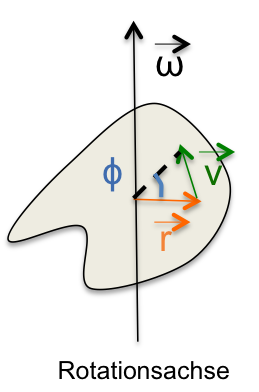
\includegraphics[width=\textwidth]{Grafik1.png}
  \caption{Rotationsbewegung}
 \end{subfigure}
 \ \ \ \ \ \ \ \ \ \ \ \ 
 \begin{subfigure}{0.16\textwidth}
  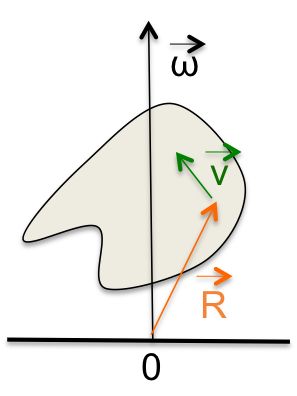
\includegraphics[width=\textwidth]{Grafik2.png}
  \caption{Vektorieller Zusammenhang zwischen $\vec{v}$, $\vec{R}$ und $\vec{\omega}$}
 \end{subfigure}  
%  \caption{Map Comparisons}
 \label{fig:mapComparisons}
\end{figure}


\newpage
\subsection{Kinetische Energie von Rotation und Translation}

\paragraph{Kinetische Energie der Translation:}Für die Translation von starren Körpern gilt

\begin{equation}
 E_{kin}^{trans} = \sum \dfrac{1}{2}m_i v_i^2 = \left(\sum \dfrac{1}{2} m_i \right) v_s^2 = \dfrac{M}{2} v_s^2
\end{equation}

 wobei wir verwendet haben, dass die Geschwindigkeit für alle Massenpunkte dieselbe ist, also $v_i = v_s$, sowie dass $\sum m_i = M$ ist. Somit erhalten wir für die Translation:
\begin{equation}
E_{kin}^{trans} = \dfrac{1}{2} M v_s^2
\end{equation}

\paragraph{Kinetische Energie der Rotation:}Für die Rotation von starren Körpern gilt 

\begin{equation}
 E_{kin}^{rot} = \sum \dfrac{1}{2} m_i v_i^2 = \sum \dfrac{1}{2} m_i r_i^2 \omega^2 = \dfrac{1}{2} I \cdot \omega^2
\end{equation}


wobei $I=\sum m_i r_i^2$ das Trägheitsmoment bezüglich einer fixen Drehachse ist. Wir haben zudem verwendet, dass $\vec{v_i}^2 = (\vec{\omega} \times \vec{r_i})^2 = r_i^2 \omega^2$. Somit erhalten wir für die Rotation:
\begin{equation}
E_{kin}^{rot} = \dfrac{1}{2} I \omega^2
\end{equation}
Hier sei Vorsicht geboten: $r_i$ bezeichnet immer den Abstand senkrecht zur Drehachse, also $r_i = R sin(\theta)$, wobei $R$ wieder der Abstand vom Ursprung zum betrachteten Punkt darstellt. Es gilt somit 

\begin{equation}
 |\vec{v}| = |\vec{\omega} \times \vec{R}| = \omega \cdot R \cdot sin(\theta) = \omega \cdot r_i
\end{equation}


Das folgende Schema soll diesen Sachverhalt veranschaulichen:

\begin{figure}[H]
  \centering{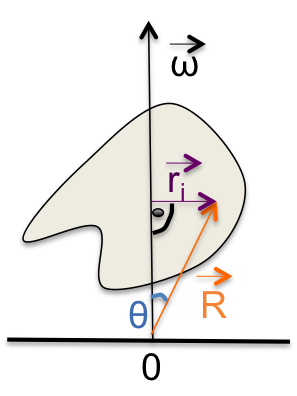
\includegraphics[width=0.3\textwidth]{Grafik3.png}}
  \label{fig:1teil}
\end{figure}

\newpage
\section{Massenträgheitsmoment}

Wie durch die Definitionen für die kinetischen Energie der Translation und der Rotation ersichtlich, gilt bei der Rotation das Massenträgheitsmoment als ähnliche Grösse zur trägen Masse bei der Translation. Das Trägheitsmoment wird immer bezüglich einer fixen Drehachse angegeben; somit ist $I_k = \sum m_i r_i^2$ das Massenträgheitsmoment bezüglich der $k$-Achse, $r_i$ gibt dabei den Abstand des i-ten Punktes zur $k$-Achse an. Es folgt eine Tabellierung von \textbf{wichtigen Massenträgheitsmomenten:}

\begin{itemize}
\item Punktmasse im Abstand $r$ um Drehachse: $I = m\cdot r^2$
\item Vollzylinder um Symmetrieachse: $I = \dfrac{1}{2}m\cdot r^2$
\item Hohlzylinder um Symmetrieachse: $I = m \dfrac{r_1^2 + r_2^2}{2}$
\item dünner Stab um Querachse: $I = \dfrac{1}{12}m \cdot l^2$
\item Vollkugel: $I = \dfrac{2}{5}m \cdot r^2$
\item Kugelschale: $I = \dfrac{2}{3}m \cdot r^2$
\end{itemize}

\paragraph{Der Satz von Steiner:}
Oft wollen wir Rotationen um Achsen betrachten, welche nicht durch den Schwerpunkt gehen. Es stellt sich nun die Frage, wie man das Trägheitsmoment für solche Rotationen berechnet.
Bezeichne $I_s$ hierbei das Trägheitsmoment bezüglich einer Drehachse, die durch den Schwerpunkt geht und $I$ das Trägheitsmoment bezüglich einer Achse, die parallel dazu läuft. Der Satz von Steiner besagt nun:
\begin{equation}
I = I_s + M \cdot s^2
\end{equation}
wobei $s$ die Distanz zwischen der betrachteten Drehachse und dem Schwerpunkt bezeichnet und $M$ die Gesamtmasse.

\begin{figure}[H]
  \centering{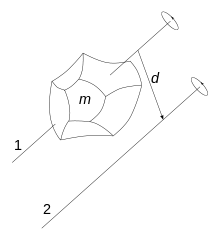
\includegraphics[width=0.3\textwidth]{steiner}}
  \caption{Situation für Satz von Steiner}
  \label{fig:stab}
\end{figure} 

\newpage
\subsection{Beispiel: Trägheitsmoment von rotierendem Stab}

\begin{figure}[H]
  \centering{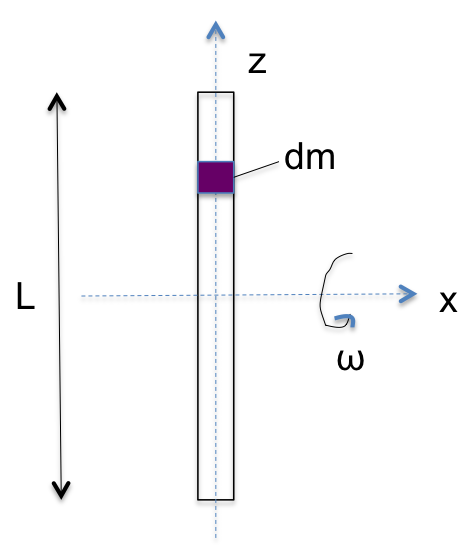
\includegraphics[width=0.2\textwidth]{Grafik4.png}}
  \caption{dünner Stab welcher um x-Achse rotiert.}
  \label{fig:stab}
\end{figure} 

Wir berechnen hier das Trägheitsmoment eines dünnen Stabes, welcher in z-Richtung liegt und sich um seine x-Achse dreht (siehe \cref{fig:stab}). Um das Trägheitsmoment zu berechnen, gehen wir von einem infinitesimalen Massenelement $dm$ aus und integrieren es über die gesamte Masse des Stabes. Also: 
\begin{equation*}
 m_i \rightarrow dm
\end{equation*}
und somit
\begin{equation*}
 I = \sum m_i r_i^2 \rightarrow \int dm \cdot r^2
\end{equation*}
Hier ist es wichtig zu beachten, zu welcher Achse wir das Trägheitsmoment berechnen wollen. Wenn wir $I_x$ haben wollen, dann gibt uns $r$ den Abstand des betrachteten (infinitesimalen) Punktes zur $x$-Achse an. Zur Berechnung werden wir folgenden Zusammenhang verwenden: 

\begin{equation*}
 dm = \rho \cdot dV = \rho \cdot dz \cdot A
\end{equation*}
wobei $A = \pi R^2$ die Querschnittsfläche des Stabes bezeichnet und $\rho$ dessen Dichte.
\begin{equation}
I_x = \int dm \cdot r^2 = \rho \int dV \cdot z^2 = \rho \pi R^2 \int_{-L/2}^{L/2} z^2  dz  = \rho \pi R^2 \cdot \left. \dfrac{z^3}{3} \right|_{-L/2}^{L/2} = \dfrac{L^3}{12} \cdot \rho \pi R^2
\end{equation}
Nun setzen wir noch die Definition der Masse eines Zylinders ein, also $M = \rho V = \rho L \pi R^2$, und erhalten für das Massenträgheitsmoment eines dünnen Stabes bezüglich der Querachse:
\begin{equation}
I_x = \dfrac{1}{12} ML^2
\end{equation}


\newpage
\section{Dynamik der Drehbewegung}
Betrachten wir das 2.Newton'sche Axiom für ein System, wobei wir nur äusseren Kräften Beachtung schenken.
\begin{equation}
\dfrac{p_i}{dt} = \vec{F_i} \rightarrow \vec{v_i} \times \dfrac{d\vec{p_i}}{dt} = \vec{r_i} \times \vec{F_i}
\end{equation}
somit folgt mit der Produktregel der Differenzialrechnung
\begin{equation}
\dfrac{d}{dt} (\vec{r_i} \times \vec{p_i}) = \dfrac{d \vec{r_i}}{dt} \times \vec{p_i} + \vec{r_i} \times \dfrac{d \vec{p_i}}{dt} = \vec{r_i} \times \dfrac{d \vec{p_i}}{dt}
\label{eq:2newton}
\end{equation}
Der erste Produktterm in \cref{eq:2newton} ist weggefallen, da $\vec{r}$ und $\vec{p}$ parallel zueinander stehen.
Wir werden nun zwei wichtige Grössen definieren:

\begin{itemize}
\item \textbf{Drehimpuls} $\vec{L_i} = \vec{r_i} \times \vec{p_i}$
\item \textbf{Drehmoment} $\vec{M_i} = \vec{r_i} \times \vec{F_i}$
\end{itemize}
Analog dazu ist der Gesamtdrehimpuls gegeben durch $\vec{L} = \sum_{i} (\vec{r_i} \times \vec{P_i})$ \\ und das Gesamtdrehmoment durch $\vec{M} = \sum_{i} (\vec{r_i} \times \vec{F_i})$

Aus diesen Definitionen und \cref{eq:2newton} folgt nun direkt der sehr nützliche \textbf{Drallsatz}:
\begin{equation}
\dfrac{d\vec{L}}{dt} = \vec{M}
\end{equation}

\paragraph{Drehimpulserhaltung:}
Der Drehimpuls ist wie der Impuls eine Erhaltungsgrösse. Dies bedeutet, dass der Gesamtdrehimpuls eines Systems zu jeder Zeit der Gleiche ist: 
\begin{equation}
 \vec{L}_{initial} =\vec{L}_{final}
\end{equation}


Formal: Wirken auf ein System von $N$ Massepunkten mit Gesamtdrehimpuls $\vec{L} = \sum_{i} \vec{L_i}$ keine äusseren Momente $\vec{M_a} = 0$, folgt unter Verwendung des Drallsatzes direkt:

\begin{equation}
\dfrac{d \vec{L}}{dt} = \vec{M_a} = 0 \quad \rightarrow \quad \vec{L} = const
\end{equation}

\newpage
\section{Rollen und Gleiten}

\subsection{Rollbedingung}
Wir wollen am Beispiel einer rotierenden Scheibe die Rollbedingung herleiten.

\begin{figure}[H]
  \centering{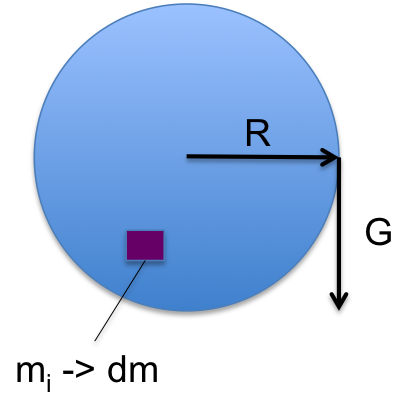
\includegraphics[width=0.15\textwidth]{Grafik5.png}}
  \label{fig:1teil}
\end{figure} 
 wobei $\vec{R}$ der Radius und $\vec{G}$ die Gewichtskraft ist. Durch diese Gewichtskraft wird auf die Scheibe ein Drehmoment ausgeübt: $\vec{M} = \vec{R} \times \vec{G}$. Da hier die Vektoren senkrecht aufeinander stehen, gilt für den Betrag $M = R \cdot G$.\\
 Betrachten wir nun den Gesamtdrehimpuls: 
 
 \begin{equation*}
   \vec{L} = \sum_{i} \vec{r_i} \times \vec{p_i} = \sum_{i} \vec{r_i} \times m_i \vec{v_i} = \sum_{i} \vec{r_i} \times \vec{e_v} m_i r_i \omega_i = \sum_{i} m_i r_i^2 \omega_i \cdot \vec{e}_{r \times v} 
 \end{equation*}
wobei $\vec{e_v}$ und $\vec{e}_{r \times v}$ Einheitsvektoren sind und wir wieder benutzt haben, dass die Vektoren senkrecht aufeinander stehen. \\\ Für starre Körper mit fester Drehachse $\vec{\omega}$ gilt $\sum_{i} m_i r_i^2 \cdot \omega = I_z \cdot \omega$ .
 Wenn wir nun den Drallsatz verwenden, erhalten wir: $\dfrac{d \vec{L}}{dt} = I \cdot \dfrac{d \omega}{dt} = M$
\\
\\
Stellen wir uns nun vor, auf dieser Scheibe sei ein Seil aufgewickelt, an welchem ein Gewicht hängt. Dann wirkt die Gewichtskraft $\vec{G}$ nach unten, das Gewicht übt eine Zugkraft $\vec{F_2}$ auf das Seil aus und vom Seil geht eine Gegenkraft $\vec{F_1}$ nach unten aus.

\begin{figure}[H]
  \centering{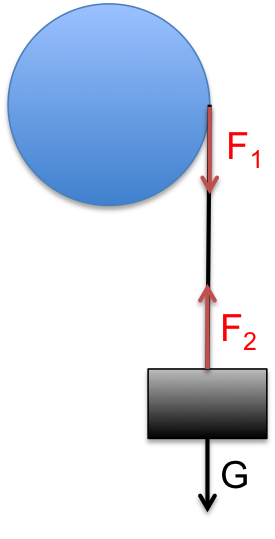
\includegraphics[width=0.15\textwidth]{Grafik6.png}}
  \label{fig:1teil}
\end{figure} 
Wir erhalten zwei Gleichungen: Eine vom fallenden Körper: $ F_2 - G = ma$, und eine von der Rotation der Scheibe: $ I \cdot \dfrac{d\omega}{dt} = R \cdot F_1$. Der Faden ist immer gestreckt, daraus erhalten wir zudem $F_1 = -F_2$. Einsetzen ergibt uns die Rollbedingung:
\begin{equation}
\vec{a} = R \cdot \dfrac{d\vec{\omega}}{dt}
\end{equation}


\subsection{Rollen auf Ebene}
\begin{figure}[H]
  \centering{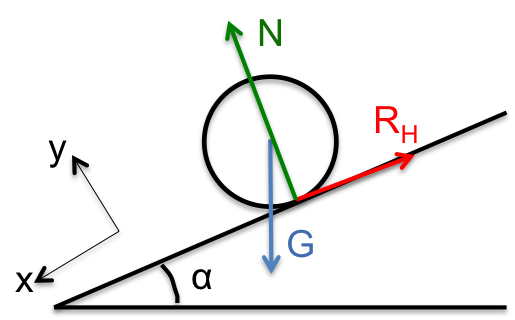
\includegraphics[width=0.4\textwidth]{Grafikrolle.png}}
  \label{fig:1teil}
\end{figure} 

\paragraph{Rollen ohne Gleiten} Wir wollen nun ein reines Rollen auf einer schiefen Ebene betrachten. Für Rollen ist eine Haftreibungskraft vonnöten, welche gegeben ist durch $R_H \leq \mu_H \cdot N$. Die Bewegungsgleichungen, aufgeteilt in Translation und Rotation, lauten nun: \\\\
\underline{Translation in x-Richtung:}
\begin{equation}
F_x = m \ddot{x_s} = Gsin(\alpha) - R_H
\end{equation}
\underline{Rotation:}
\begin{equation}
M = \dfrac{dL}{dt} = I_z \dfrac{d \omega}{dt} = r \cdot R_H \\\\
\end{equation}
Hier haben wir genutzt, dass die Kraft $R_H$ senkrecht zu $r$ steht. Wenn wir nun die Rollbedinung benutzen, erhalten wir:
\begin{equation}
a = \ddot{x_s} = r \dfrac{d \omega}{dt} = r^2 \dfrac{R_H}{I_z} = \dfrac{r^2}{I_z} (G sin(\alpha) - m \ddot{x_s}) = \dfrac{m r^2}{I_z} (g \cdot sin(\alpha) - \ddot{x_s})
\end{equation}
somit erhalten wir durch Umformen
\begin{equation}
\ddot{x_s} = \dfrac{g \cdot sin(\alpha)}{1 + \dfrac{I_z}{mr^2}}
\end{equation}
Wir sehen also, dass wenn zwei Körper gleicher Masse und mit gleichem Radius unterschiedlich schnell rollen, müssen sie unterschiedliche Massenträgheitsmomente haben.  Die innere Verteilung der Massenpunkte spielt beim Rollvorgang somit eine wichtige Rolle.

% 
% \paragraph{Rollen mit Gleiten}
% Betrachten wir nun noch den Fall eines Zylinders, der sich bereits im rotierenden Zustand befinden, wenn er auf die schräge Ebene aufgesetzt wird. (Es ist die gleiche Grafik zu betrachten, nur das nun der Körper zu Beginn schon eine Rotationgeschwindigkeit hat.)\\
% Es gilt: $I_z = \dfrac{1}{2} mr^2$ für Zylinder, $M = \dfrac{dL}{dt} = I_z \cdot \dfrac{d \omega}{dt} = -r \cdot R_G$ das Minus kommt daher, dass die Reibungskraft ja in negative x-Richtung zeigt. Wenn wir uns die Kräfte anschauen bekommen wir folgende Bewegungsgleichungen für die Translation in x- und y-Richtung:
% \begin{equation}
% m \ddot{x_s} = Gsin(\alpha) -R_G
% \end{equation}
% \begin{equation}
% m \ddot{y_s} = -Gcos(\alpha) + N = 0
% \end{equation}
% \clearpage
% aus den vorhergehenden Gleichungen und Überlegungen erhalten wir folgende Relationen:\\
% $N = Gcos(\alpha)$\\
% $R_G = \mu_G N = \mu_G G cos(\alpha)$\\
% $I_z \dot{\omega} + rR_G = 0 \rightarrow \omega = \omega_0 - \dfrac{\mu_G G cos(\alpha)r}{I_z} \cdot t$ ($\omega_o$ ist einfach die Anfangswinkelgeschwindigkeit vor dem Aufsetzen)\\
% Verwenden wir die Anfangsbedingungen $x_s(0) = 0$ und $v_s(0) = 0$ bekommen wir für die Geschwindigkeit in x-Richtung:
% \begin{equation}
% v_x = g\cdot (sin(\alpha) - \mu_G cos(\alpha)) \cdot t
% \end{equation}
% Daraus ergeben sich nun drei Fälle:\\
% \\
% \textbf{Fall 1}: $\mu_G > tan(\alpha) \rightarrow$ Zylinder bewegt sich nach oben.\\
% \textbf{Fall 2}: $\mu_G < tan(\alpha) \rightarrow$ Zylinder bewegt sich nach unten.\\
% \textbf{Fall 3}: $\mu_G = tan(\alpha) \rightarrow$ Zylinder rotiert an Ort und Stelle.
\end{document}